\documentclass{jsarticle}
\title{ほげほげ}
\author{author name}
\date{} % 指定したければ文字列を入れる 削除するとコンパイル日付が入る

\usepackage[dvipdfmx, bookmarks=true, bookmarksnumbered=true, colorlinks=true, linkcolor=black]{hyperref} % 目次からジャンプ可能にする colorlinksを付けないと赤枠で囲われる(cygwin)
\usepackage[dvipdfmx]{graphicx, color} % 画像を入れる
\usepackage[top=20truemm, bottom=20truemm, left=25truemm, right=25truemm]{geometry} % 描画範囲指定
\usepackage{float} % 位置指定[H]で位置を強制する
\usepackage{ifthen} % ifthenelseを使う

\usepackage{hoge} % 同フォルダに配置したhoge.styを読む

\begin{document}
\maketitle % タイトルを表示
\tableofcontents % 目次を表示

\section{\LaTeX}
\subsection{箇条書き}

\begin{enumerate}
\item 数字付き
\end{enumerate}

\begin{itemize}
\item 箇条書き
\item 
\item [hoge] [hoge]で指定
\item [fuga]
\item [] []で点を表示しない
\item end
\end{itemize}

\subsection{minipage, figure}

\begin{table}[H]
  \begin{minipage}{.5\textwidth}
    \begin{figure}[H]
      \centering
      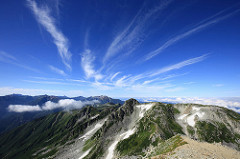
\includegraphics[width=200pt]{sample.png}
      \caption{sample}
    \end{figure}
  \end{minipage}
  \begin{minipage}{.5\textwidth}
    minipageの改行も\verb|\\|で可能
  \end{minipage}
\end{table}

\subsubsection{これは目次に表示されない}

\hoge % hoge.sty で定義されたコマンド

\tablefigure{a}

\tablefigure{2}

\tablefigure{3}

\newpage % 改ページ

\thispagestyle{empty} % ページ番号を表示しない(カウントはされる)

\section{Emacs}
\subsection{Emacsコマンド}
$< $C-x$>< $C-e$>$ で $\backslash $end\{hogehoge\}を\verb|\|begin\{hogehoge\}に合わせて出力

\begin{itemize}
\item C-M-m で \textbackslash item を出力
\end{itemize}

\clearpage % 図表を全て出力して改ページ

\section{Vim}
Vimについて
 % vim.tex の内容を呼び出す

\end{document}
